\documentclass{article}
\usepackage{graphicx} % Required for inserting images
\usepackage{subcaption}
\usepackage{hyperref}
\usepackage{caption}
\usepackage{float}
\usepackage{amsmath}
\usepackage[italian]{babel}

\title{
    \Huge{Architetture dati}\\
    \Huge{\textbf{Errori nei dati di training: impatto sui modelli ML}}\\[1cm]

    {\Large
    \begin{tabular}{rl}
        Tommaso Baggio & matricola 912356 \\
        Samuele Bergamin & matricola 844861 \\
        Andrea Ciacci & matricola 899883 \\
    \end{tabular}
    } \\[3cm]
    
    
\includegraphics[width=6cm]{Immagini/Logo bicocca.jpg}\\[1cm] 
    \author{}
    \Large{Anno accademico 2025-2026}
}
\date{}


\begin{document}

\maketitle
\newpage

\tableofcontents
\newpage

\section{Introduzione}

Il nostro progetto tratta di come l'aggiunta di rumore nei dataset influisca sulle performance dei modelli di Machine Learning, prendendo come spunto principale per l’idea il paper “Impact of Noise in Dataset on Machine Learning Algorithms” (Saseendran, Arun Thundyill, et al, Mach. Learn. Res 1 (2019): 1-8) \hyperlink{https://www.researchgate.net/profile/Arun-Saseendran-2/publication/331024938_Impact_of_Noise_in_Dataset_on_Machine_Learning_Algorithms/links/5c61eff8a6fdccb608bba512/Impact-of-Noise-in-Dataset-on-Machine-Learning-Algorithms.pdf}{(repribile qui)}.\\
L’obiettivo principale consiste nel verificare e giustificare le differenze tra i risultati ottenuti sui dataset originali e sui dataset sporcati. \\
Per fare ciò, analizziamo 3 dataset distinti, li sporcheremo, e successivamente per ognuno addestreremo 3 diversi modelli: in questo modo, potremo poi confrontare i vari risultati.

\subsection{Datasets}

Per questo progetto sono stati scelti tre dataset, reperibili su \hyperlink{https://www.kaggle.com/}{Kaggle}.\\
L'analisi viene ripetuta su tre dataset con caratteristiche molto diverse:
\begin{enumerate}
    \item \textbf{Teen Mental Health Dataset}, piccolo e fortemente sbilanciato;
    \item \textbf{Adult Income Dataset}, più grande e con numerose variabili categoriche;
    \item \textbf{Liver Patient Dataset}, piccolo, clinico e caratterizzato da forti outlier.
\end{enumerate}

Le variabili categoriche vengono codificate con one-hot encoding.\\

Il dataset viene prima diviso in training+validation e test mediante uno split stratificato. Il blocco training+validation viene poi diviso nuovamente, sempre in modo stratificato. Nel flusso principale le proporzioni sono circa:
\[
70\%\ \text{training}, \qquad 15\%\ \text{validation}, \qquad 15\%\ \text{test}.
\]
Il training serve per stimare i parametri del modello. La validation serve per scegliere profondità, potatura e pesi di classe. Il test viene consultato solo dopo la selezione. Questa modifica elimina il \textit{test leakage}: scegliere gli iperparametri sul test renderebbe la valutazione finale eccessivamente favorevole.

\newpage

\subsection{Aggiunta del rumore}
La nostra strategia consiste nell'andare a modificare le righe originali. A differenza dell'articolo, però, andiamo a modificare solamente il training set, lasciando intatto il test set.\\
Il rumore viene aggiunto progressivamente, dallo $0\%$ a $100\%$ di righe modificate, con step di $10\%$.\\
Il rumore viene applicato diversamene in base al tipo di feature:
\begin{itemize}

    \item \textbf{Variabili categoriche}: 
    Avendo codificato le variabili categoriche in one-hot, la strategia di corruzione consiste nel disattivare la colonna corrispondente alla categoria a cui faceva parte in origine la riga, e attivarne un’altra;
        \item \textbf{Variabili continue}: 
    La funzione \texttt{corrupt\_rows\_cont} introduce invece rumore additivo gaussiano sulle variabili numeriche. Anche in questo caso viene selezionata una frazione \( \rho \) delle righe del training set, e per ciascun valore selezionato si applica una perturbazione del tipo:
    \[
    \tilde{x}_i = x_i + \epsilon, \quad \epsilon \sim \mathcal{N}(0, \sigma^2)
    \]
    
    dove la deviazione standard del rumore è definita come:
    \[
    \sigma = \texttt{noise\_level} \cdot \mathrm{std}(X_{\cdot j})
    \]
    
    in cui \( \mathrm{std}(X_{\cdot j}) \) rappresenta la deviazione standard empirica della colonna considerata. Questo rende il rumore adattivo alla scala della variabile, evitando distorsioni non proporzionate.
    \item \textbf{Variabili intere e ordinali}:  In questo caso, scegliamo una variazione locale da applicare, ad esempio, -2, -1, 0, 1, 2, e il risultato viene mantenuto entro limiti espliciti.
\end{itemize}
    Come valore di \texttt{noise\_level}, dopo aver sperimentato con diveersi valori, abbiamo scelto di usare 0.5.


    Come metodo di applicazione, le feature sono state ordinate in base al valore di Mutual Information rispetto alla variabile target e successivamente suddivise in due gruppi: il primo contenente le feature con Mutual Information più elevata e il secondo quelle con valori inferiori. Il rumore è stato applicato separatamente a ciascun gruppo, mantenendo inalterato l'altro, al fine di valutare come la perturbazione delle feature più o meno informative influenzi le prestazioni del modello.
    \\



\newpage
\subsection{Metriche}

Indicando con TP, TN, FP e FN gli elementi della matrice di confusione, vengono calcolate:

\begin{flalign*}
&\text{Accuracy} = \frac{TP+TN}{TP+TN+FP+FN},&\\
&\text{Recall}_1 = \frac{TP}{TP+FN},&\\
&\text{Precision}_1 = \frac{TP}{TP+FP},&\\
&F1_1 = 2\frac{\text{Precision}_1\,\text{Recall}_1}
{\text{Precision}_1+\text{Recall}_1},&\\
&\text{Balanced Accuracy} = \frac{1}{2}
\left(\frac{TP}{TP+FN}+\frac{TN}{TN+FP}\right).&
\end{flalign*}



\subsection{Modelli ML}
\subsubsection{Decision Tree}

Il primo modello che abbiamo preso in considerazione è il Decision Tree, in quanto dà risultati interpretabili e ottiene una elevata velocità di addestramento e inferenza.\\
Per contenere l'overfitting abbiamo introdotto due meccanismi principali:
\begin{itemize}
    \item Il primo è la limitazione della profondità massima tramite il parametro \texttt{max\_depth}, che ne limita la complessità;
    \item Il secondo è il \textit{cost-complexity pruning}, che penalizza la complessità strutturale dell'albero introducendo il parametro $\alpha$ nella funzione obiettivo:

    \begin{equation}
        \mathcal{L}_\alpha(T) = \text{errore}(T) + \alpha \cdot |T|
    \end{equation}

    dove $|T|$ indica il numero di foglie dell'albero $T$.
    Valori più elevati di $\alpha$ producono alberi più potati e quindi più semplici.
    \item infine vi è il class\_weight, il quale gestisce lo sbilanciamento fra le classi. 
\end{itemize}

La scelta dei valori ottimali per queste variabili avviene tramite una ricerca a griglia sui valori candidati, selezionando la configurazione
che massimizza la metrica scelta sul test set.\\
Ogni configurazione produce un ensemble di tre alberi. Ciascun albero viene addestrato sui due fold di training di una suddivisione stratificata a tre fold, cioè su circa il 66\% del training set.

\subsubsection{Neural Network}

Il secondo modello addestrato per ciascun dataset è una rete neurale, scelta per la sua capacità di apprendere rappresentazioni complesse dei dati e modellare relazioni non lineari tra le variabili.\\
Per la fase di normalizzazione è stato utilizzato \texttt{RobustScaler()} (dalla libreria \texttt{sklearn}), ritenuto più adatto alla struttura dei dataset rispetto ad altri metodi di scaling come \texttt{StandardScaler()}. A differenza della standardizzazione basata su media e deviazione standard, \texttt{RobustScaler} utilizza la mediana e l'intervallo interquartile (IQR), risultando meno sensibile alla presenza di valori anomali (\textit{outlier}).\\
Per le reti abbiamo usato la libreria \texttt{tensorflow} e  \texttt{keras}.\\
La funzione \texttt{build\_model(input\_dim)} si occupa della costruzione della rete neurale, definendo un'architettura composta da tre livelli densi con rispettivamente 32, 16 e 1 neurone. L'ultimo livello è il singolo neurone di output, e utilizza una funzione di attivazione sigmoide, poiché i dataset affrontano un problema di classificazione binaria e l'output rappresenta una probabilità compresa tra 0 e 1.\\
Nei test progressivi vengono usati:
\begin{itemize}
    \item bootstrap del training per diversificare i modelli;
    \item pesi di classe calcolati sul training;
    \item early stopping sulla validation loss;
    \item media delle probabilità dei modelli e soglia 0.5;
    \item ripetizioni con seed controllati e deviazione standard delle metriche.
\end{itemize}


\newpage
\subsubsection{SVM}
Il terzo modello utilizzato per ciascun dataset è una Support Vector Machine (SVM). Abbiamo deciso di adottare il kernel RBF (Radial Basis Function), che consente al modello di proiettare implicitamente i dati in uno spazio di dimensione superiore, rendendo possibile la separazione anche in presenza di relazioni non lineari tra le variabili.\\
Per la normalizzazione dei dati è stato utilizzato nuovamente RobustScaler().
L'implementazione è stata realizzata tramite la libreria \texttt{scikit-learn}, utilizzando la classe \texttt{SVC}. 
Il modello è stato configurato con il parametro \texttt{class\_weight = "balanced"}, al fine di compensare eventuali squilibri tra le classi e ridurre il rischio di bias verso la classe maggioritaria, soprattutto in condizioni di elevato rumore nei dati. Inoltre, è stato utilizzato \texttt{gamma = "scale"}, che imposta il valore di gamma a
\[
\frac{1}{n_{\text{features}} \cdot X.\mathrm{var}()}
\]
e \texttt{C = 1} come parametro di regolarizzazione.
Per ciascun livello di rumore vengono costruiti tre modelli su campioni bootstrap. La predizione finale è ottenuta mediante voto di maggioranza sulle classi predette.

Per questo modello, pur non avendo inserito parametri da ottimizzare, è stato effettuato lo split per il validation set per omogeneità con gli altri modelli.

\newpage


\section{Liver Patient Dataset}

Il dataset raccoglie informazioni cliniche di pazienti provenienti dalla regione nord-orientale dell'Andhra Pradesh, in India. Le variabili incluse descrivono caratteristiche demografiche e parametri biochimici correlati alla funzionalità del fegato. Grazie alla presenza di una variabile target che indica la presenza o meno di una malattia epatica, il dataset rappresenta un valido strumento per studi di classificazione e analisi predittiva in ambito medico.

\subsection{Descrizione dataset}

Il dataset è composto da \textbf{11 colonne} e \textbf{583 righe}.

\begin{table}[htbp]
\centering
\label{tab:featuresLiver}
\begin{tabular}{ll}
\hline
\textbf{Nome Variabile} & \textbf{Descrizione} \\
\hline
age & Età del paziente \\
gender & Genere \\
TB & Livello di bilirubina totale \\
DB & Livello di bilirubina diretta \\
alkphos & Livello dell'enzima epatico fosfatasi alcalina \\
sgpt & Alanina Aminotransferasi (ALT) \\
sgot & Aspartato Aminotransferasi (AST) \\
TP & Livello di proteine totali \\
ALB & Livello di albumina \\
a/g ratio & Rapporto Albumina/Globuline \\
Selector & Variabile target (classe di appartenenza) \\
\hline
\end{tabular}
\end{table}

La distribuzione del target è: \textbf{71\% positivi, 29\% negativi}.

\begin{figure}[H]
    \centering
    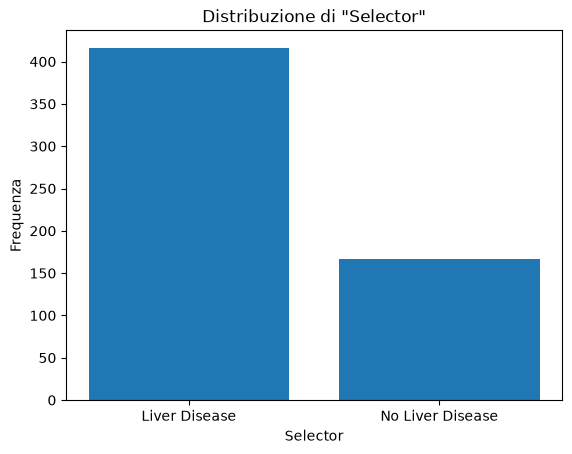
\includegraphics[width=0.7\linewidth]{Immagini/Liver/distribuzioneTargetLiver.png}
    \label{fig:distribuzioneTargetLiver}
\end{figure}

Attraverso il calcolo della Mutual Information per le varie feature, otteniamo una classifica, dalla più importante alla meno importante.

\begin{figure}[H]
    \centering
    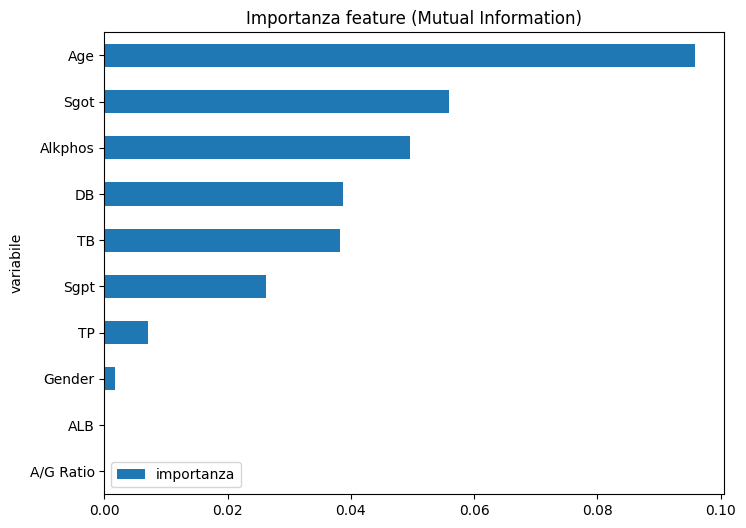
\includegraphics[width=1\linewidth]{Immagini/Liver/MILiver.png}
    \label{fig:importanzaFeatureliver}
\end{figure}


\subsection{Risultati}
Dalla Mutual Information, otteniamo le 2 metà di feature:
\begin{itemize}
    \item \textbf{Peggiori}: ['Sgpt', 'TP', 'Gender', 'ALB', 'A/G Ratio'].;
    \item \textbf{Migliori}: ['Age', 'Sgot', 'Alkphos', 'DB', 'TB'].

\end{itemize}

\newpage
 
\subsubsection{Decision Tree}


\begin{figure}[H]
    \centering
    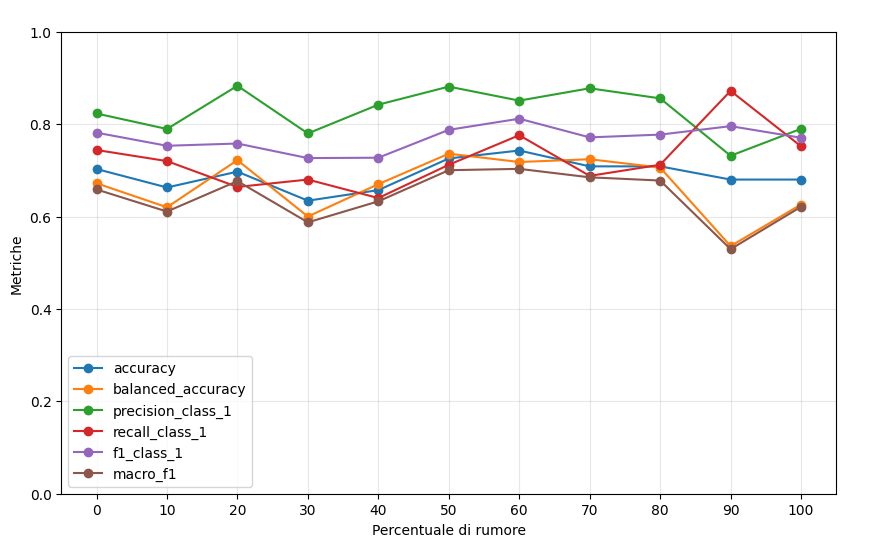
\includegraphics[width=1\linewidth]{Immagini/Liver/RobustezzaEnsemble.png}
    \label{fig:robustezza-ensemble-decision-tree-liver}
\end{figure}

\begin{table}[ht]
\centering
\begin{tabular}{cccccc}
\hline
\textbf{\% Rumore} & \textbf{Accuracy} & \textbf{Balanced Acc.} & \textbf{Precision} & \textbf{Recall} & \textbf{F1} \\
\hline
0   & 0.703 & 0.672 & 0.823 & 0.744 & 0.782 \\
10  & 0.663 & 0.620 & 0.789 & 0.720 & 0.753 \\
20  & 0.697 & 0.722 & 0.883 & 0.664 & 0.758 \\
30  & 0.634 & 0.600 & 0.780 & 0.680 & 0.726 \\
40  & 0.657 & 0.670 & 0.842 & 0.640 & 0.727 \\
50  & 0.726 & 0.736 & 0.881 & 0.712 & 0.788 \\
60  & 0.743 & 0.718 & 0.851 & 0.776 & 0.812 \\
70  & 0.709 & 0.724 & 0.878 & 0.688 & 0.771 \\
80  & 0.709 & 0.706 & 0.856 & 0.712 & 0.777 \\
90  & 0.680 & 0.536 & 0.732 & 0.872 & 0.796 \\
100 & 0.680 & 0.626 & 0.790 & 0.752 & 0.770 \\
\hline
\end{tabular}
\caption{Risultati ottenuti dal Decision Tree sporcando le feature peggiori}
\label{tab:prestazioni_feature_peggiori}
\end{table}

\begin{figure}[H]
    \centering
    
\includegraphics[width=1\linewidth]{Immagini/Liver/RobustezzaEnsembleMigliori.png}
    \label{fig:robustezza-ensemble-decision-tree-liver-migliori}
\end{figure}

\begin{table}[ht]
\centering
\begin{tabular}{cccccc}
\hline
\textbf{\% Rumore} & \textbf{Accuracy} & \textbf{Balanced Acc.} & \textbf{Precision} & \textbf{Recall} & \textbf{F1} \\
\hline
0   & 0.703 & 0.672 & 0.823 & 0.744 & 0.782 \\
10  & 0.697 & 0.686 & 0.840 & 0.712 & 0.771 \\
20  & 0.674 & 0.664 & 0.827 & 0.688 & 0.751 \\
30  & 0.657 & 0.568 & 0.752 & 0.776 & 0.764 \\
40  & 0.657 & 0.622 & 0.793 & 0.704 & 0.746 \\
50  & 0.686 & 0.708 & 0.872 & 0.656 & 0.749 \\
60  & 0.629 & 0.632 & 0.813 & 0.624 & 0.706 \\
70  & 0.577 & 0.566 & 0.763 & 0.592 & 0.667 \\
80  & 0.657 & 0.568 & 0.752 & 0.776 & 0.764 \\
90  & 0.634 & 0.684 & 0.877 & 0.568 & 0.689 \\
100 & 0.594 & 0.620 & 0.814 & 0.560 & 0.664 \\
\hline
\end{tabular}
\caption{Risultati ottenuti dal Decision Tree sporcando le feature migliori}
\label{tab:prestazioni_feature_migliori}
\end{table}
\newpage
\subsubsection{Neural Network}


\begin{figure}[H]
    \centering
    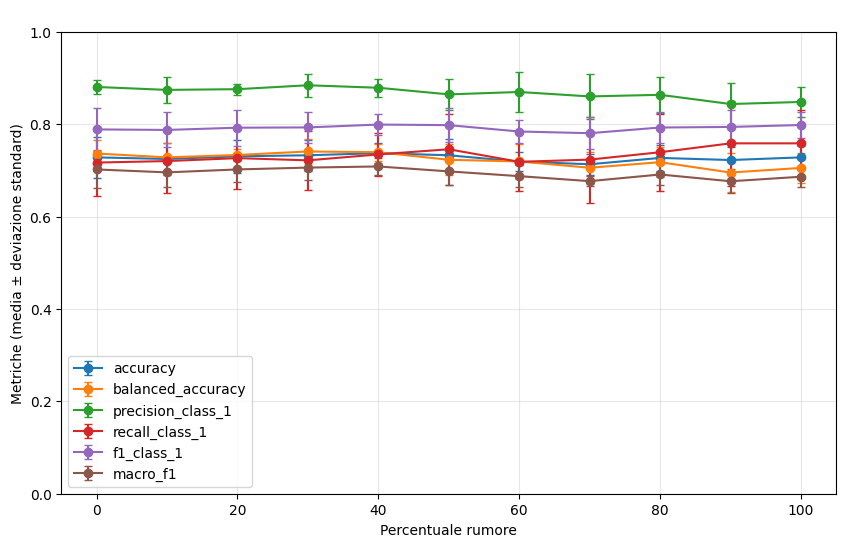
\includegraphics[width=1\linewidth]{Immagini/Liver/RobustezzaNNEnsemble.png}
    \label{fig:robustezza-nn-ensemble-liver-peggiori}
\end{figure}

\begin{table}[H]
\centering
\label{tab:feat_peggiori}
\begin{tabular}{ccccccc}
\hline
\textbf{\% Rumore} & \textbf{Accuracy} & \textbf{Balanced Acc.} & \textbf{Precision} & \textbf{Recall} & \textbf{F1} \\
\hline
0   & 0.6229 & 0.706 & 0.9275 & 0.512 & 0.6598 \\
10  & 0.6229 & 0.712 & 0.9403 & 0.504 & 0.6562 \\
20  & 0.6229 & 0.706 & 0.9275 & 0.512 & 0.6598 \\
30  & 0.6571 & 0.736 & 0.9452 & 0.552 & 0.6970 \\
40  & 0.6171 & 0.702 & 0.9265 & 0.504 & 0.6529 \\
50  & 0.6457 & 0.722 & 0.9315 & 0.544 & 0.6869 \\
60  & 0.6286 & 0.710 & 0.9286 & 0.520 & 0.6667 \\
70  & 0.6343 & 0.720 & 0.9420 & 0.520 & 0.6701 \\
80  & 0.6457 & 0.722 & 0.9315 & 0.544 & 0.6869 \\
90  & 0.6286 & 0.710 & 0.9286 & 0.520 & 0.6667 \\
100 & 0.6229 & 0.718 & 0.9538 & 0.496 & 0.6526 \\
\hline
\end{tabular}
\caption{Risultati ottenuti dalla Neural Network sporcando le feature peggiori}
\end{table}


\begin{figure}[H]
    \centering
    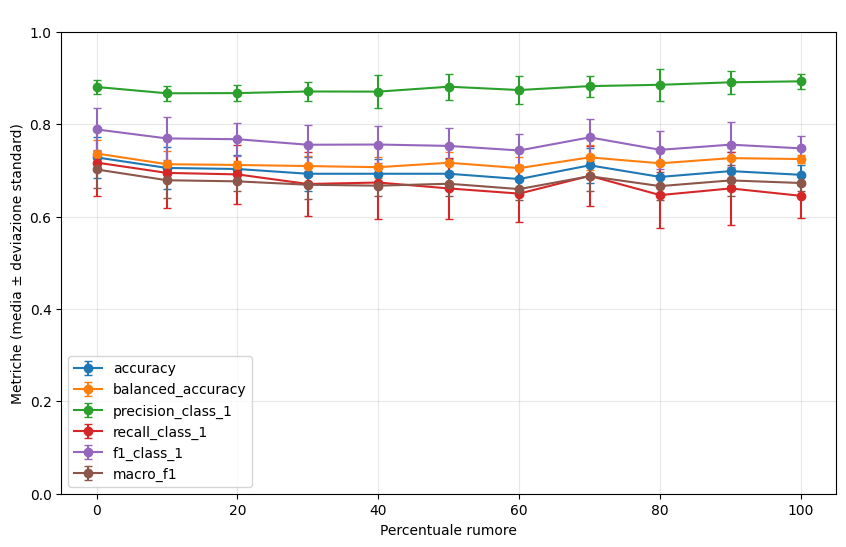
\includegraphics[width=1\linewidth]{Immagini/Liver/RobustezzaNNEnsembleMigliori.png}
    \label{fig:robustezza-nn-ensemble-liver-migliori}
\end{figure}


\begin{table}[ht]
\centering
\begin{tabular}{cccccc}
\hline
\textbf{\% Rumore} & \textbf{Accuracy} & \textbf{Balanced Acc.} & \textbf{Precision} & \textbf{Recall} & \textbf{F1} \\
\hline
0   & 0.6229 & 0.706 & 0.9275 & 0.512 & 0.6598 \\
10  & 0.6229 & 0.712 & 0.9403 & 0.504 & 0.6562 \\
20  & 0.6229 & 0.706 & 0.9275 & 0.512 & 0.6598 \\
30  & 0.6571 & 0.736 & 0.9452 & 0.552 & 0.6970 \\
40  & 0.6171 & 0.702 & 0.9265 & 0.504 & 0.6529 \\
50  & 0.6457 & 0.722 & 0.9315 & 0.544 & 0.6869 \\
60  & 0.6286 & 0.710 & 0.9286 & 0.520 & 0.6667 \\
70  & 0.6343 & 0.720 & 0.9420 & 0.520 & 0.6701 \\
80  & 0.6457 & 0.722 & 0.9315 & 0.544 & 0.6869 \\
90  & 0.6286 & 0.710 & 0.9286 & 0.520 & 0.6667 \\
100 & 0.6229 & 0.718 & 0.9538 & 0.496 & 0.6526 \\
\hline
\end{tabular}
\caption{Risultati ottenuti dalla Neural Network sporcando le feature migliori}
\label{tab:prestazioni_feature_migliori}
\end{table}



\subsubsection{SVM}


\begin{figure}[H]
    \centering
    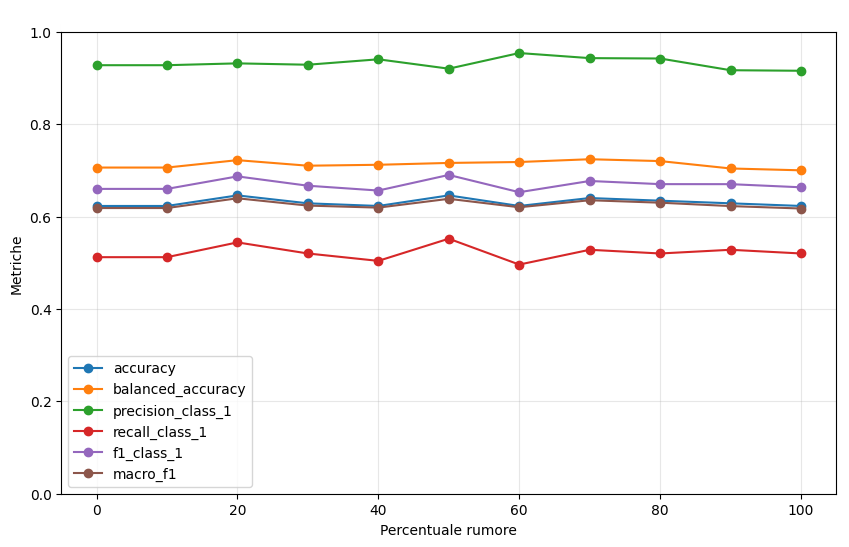
\includegraphics[width=1\linewidth]{Immagini/Liver/RobustezzaSVMEnsemble.png}
    \label{fig:robustezza-svm-ensemble-liver-peggiori}
\end{figure}

\begin{table}[ht]
\centering
\begin{tabular}{cccccc}
\hline
\textbf{\% Rumore} & \textbf{Accuracy} & \textbf{Balanced Acc.} & \textbf{Precision} & \textbf{Recall} & \textbf{F1} \\
\hline
0   & 0.606 & 0.700 & 0.414 & 0.920 & 0.571 \\
10  & 0.617 & 0.714 & 0.423 & 0.940 & 0.584 \\
20  & 0.606 & 0.700 & 0.414 & 0.920 & 0.571 \\
30  & 0.606 & 0.700 & 0.414 & 0.920 & 0.571 \\
40  & 0.606 & 0.694 & 0.413 & 0.900 & 0.566 \\
50  & 0.617 & 0.702 & 0.421 & 0.900 & 0.573 \\
60  & 0.629 & 0.710 & 0.429 & 0.900 & 0.581 \\
70  & 0.629 & 0.716 & 0.430 & 0.920 & 0.586 \\
80  & 0.611 & 0.704 & 0.418 & 0.920 & 0.575 \\
90  & 0.646 & 0.716 & 0.440 & 0.880 & 0.587 \\
100 & 0.611 & 0.692 & 0.415 & 0.880 & 0.564 \\
\hline
\end{tabular}
\caption{Risultati ottenuti dalla SVM sporcando le feature peggiori}
\label{tab:prestazioni_feature_peggiori_SVM_liver}
\end{table}


\begin{figure}[H]
    \centering
    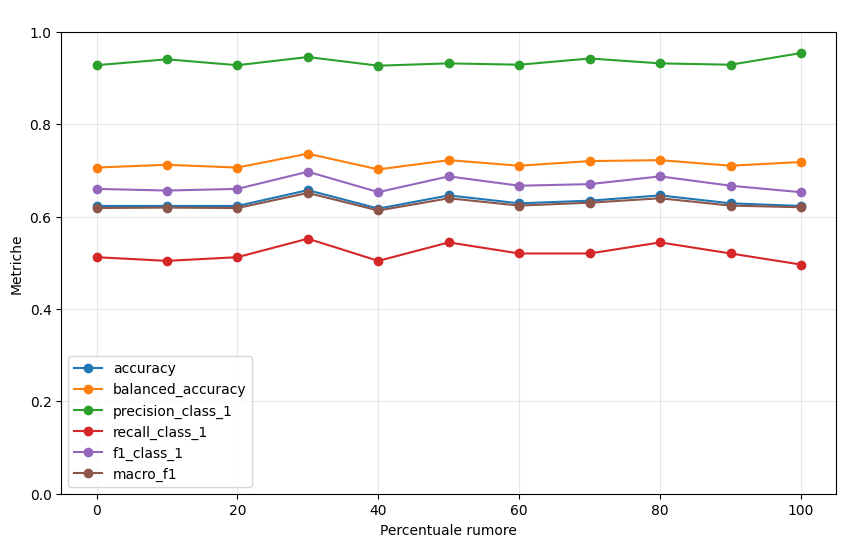
\includegraphics[width=1\linewidth]{Immagini/Liver/RobustezzaSVMEnsembleMigliori.png}
    \label{fig:robustezza-svm-ensemble-liver-migliori}
\end{figure}

\begin{table}[ht]
\centering
\begin{tabular}{cccccc}
\hline
\textbf{\& Rumore} & \textbf{Accuracy} & \textbf{Balanced Acc.} & \textbf{Precision} & \textbf{Recall} & \textbf{F1} \\
\hline
0   & 0.606 & 0.700 & 0.414 & 0.920 & 0.571 \\
10  & 0.623 & 0.712 & 0.426 & 0.920 & 0.582 \\
20  & 0.606 & 0.700 & 0.414 & 0.920 & 0.571 \\
30  & 0.606 & 0.694 & 0.413 & 0.900 & 0.566 \\
40  & 0.623 & 0.700 & 0.423 & 0.880 & 0.571 \\
50  & 0.611 & 0.692 & 0.415 & 0.880 & 0.564 \\
60  & 0.606 & 0.700 & 0.414 & 0.920 & 0.571 \\
70  & 0.611 & 0.698 & 0.417 & 0.900 & 0.570 \\
80  & 0.634 & 0.702 & 0.430 & 0.860 & 0.573 \\
90  & 0.606 & 0.688 & 0.411 & 0.880 & 0.561 \\
100 & 0.634 & 0.702 & 0.430 & 0.860 & 0.573 \\
\hline
\end{tabular}
\caption{Risultati ottenuti dalla SVM sporcando le feature migliori}
\label{tab:prestazioni_feature_migliori_SVM_liver}
\end{table}



\newpage


\section{Teen Mental Health Dataset}

Il dataset raccoglie informazioni relative alla salute mentale degli adolescenti, includendo variabili comportamentali, psicologiche e legate allo stile di vita. Tra queste rientrano l’uso dei social media, la durata del sonno, il rendimento scolastico e i livelli di stress, ansia e depressione.
\\
L’obiettivo principale dei dati è permettere l’analisi delle relazioni tra abitudini quotidiane e condizioni di benessere mentale, evidenziando possibili fattori di rischio o correlazioni significative.

\subsection{Descrizione dataset}
Il dataset è composto da \textbf{13 colonne} e \textbf{1200 righe}.

\begin{table}[htbp]
\centering
\label{tab:featuresAdult2}
\begin{tabular}{ll}
\hline
\textbf{Nome Variabile} & \textbf{Descrizione} \\
\hline 
age & Età dell’individuo \\
gender & Genere \\
daily\_social\_media\_hours & Ore passate sui social \\
platform\_usage & Piattaforma social usata, tra Instagramm e TikTok \\
sleep\_hours & Ore di sonno \\
screen\_time\_before\_sleep & Tempo passato davanti allo schermo prima di dormire \\
physical\_activity & Ore di attività fisica \\
social\_interaction\_level & Livello di interazione sociale \\
stress\_level & Livello di stress \\
anxiety\_level & Livello d'ansia \\
addiction\_level & Livello di dipendenza \\
depression\_label & Diagnosi di depressione \\
\hline
\end{tabular}
\end{table}

La distribuzione del target è: \textbf{97,46\% negativi, 2,58\% positivi}.

\begin{figure}[H]
    \centering
    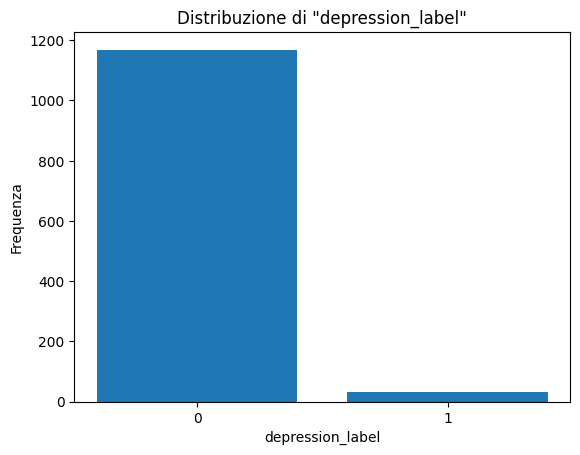
\includegraphics[width=0.7\linewidth]{Immagini/Teen/DistribuzioneTargetTeen.png}
    \label{fig:DistribuzioneTargetTeen}
\end{figure}
\newpage


Attraverso il calcolo della Mutual Information per le varie feature, otteniamo una classifica, dalla più importante alla meno importante.

\begin{figure}[H]
    \centering
    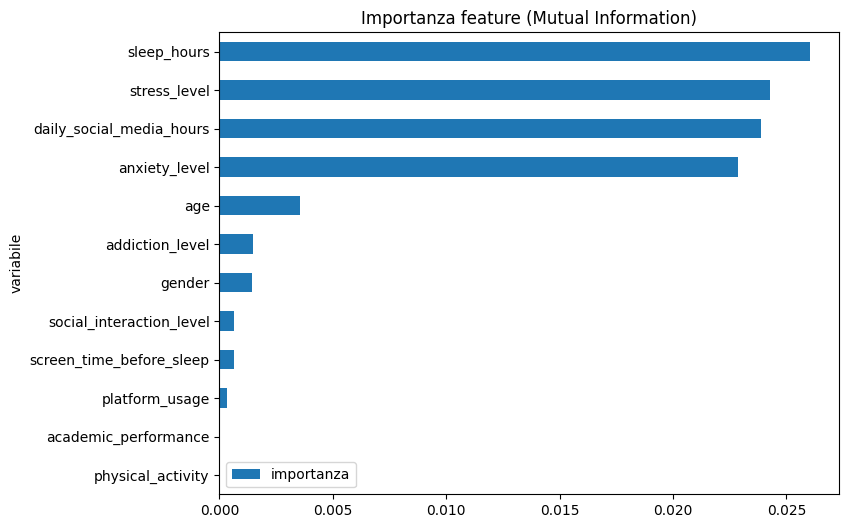
\includegraphics[width=1\linewidth]{Immagini/Teen/MITeen.png}
    \label{fig:MITeen}
\end{figure}


\subsection{Risultati}

Abbiamo diviso le feature in 2 metà in base alla Mutual Information:
\begin{itemize}
    \item \textbf{Peggiori}: ['gender', 'social\_interaction\_level', 'screen\_time\_before\_sleep', 'platform\_usage', 'academic\_performance', 'physical\_activity']
    \item \textbf{Migliori}:['sleep\_hours', 'stress\_level', 'daily\_social\_media\_hours', 'anxiety\_level', 'age', 'addiction\_level'].
\end{itemize}

Per ogni modello, abbiamo sporcato progressivamente il dataset e monitorato le prestazioni.
\newpage

\subsubsection{Decision Tree}

\begin{figure}[H]
    \centering
    \makebox[\textwidth][c]{%
        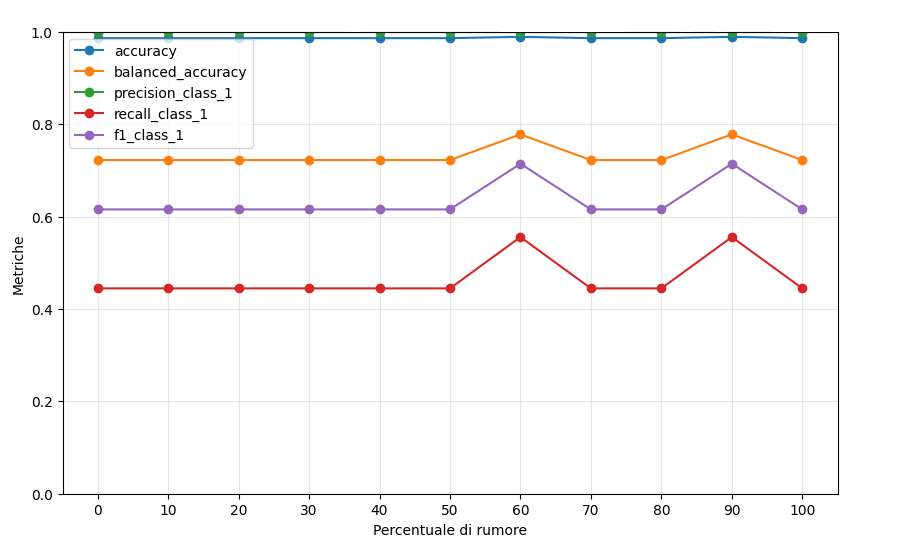
\includegraphics[width=1\linewidth]{Immagini/Teen/RobustezzaEnsamble1teen.png}%
    }
    \label{fig:alberiPeggioriDCTeen}
\end{figure}



\begin{table}[htbp]
\centering
\label{tab:rumore_risultati1}
\begin{tabular}{cccccc}
\hline
\textbf{\% Rumore} & \textbf{Accuracy} & \textbf{Balanced Acc.} & \textbf{Precision} & \textbf{Recall} & \textbf{F1} \\
\hline
0   & 0.9861 & 0.7222 & 1.0000 & 0.4444 & 0.6154 \\
10  & 0.9861 & 0.7222 & 1.0000 & 0.4444 & 0.6154 \\
20  & 0.9861 & 0.7222 & 1.0000 & 0.4444 & 0.6154 \\
30  & 0.9861 & 0.7222 & 1.0000 & 0.4444 & 0.6154 \\
40  & 0.9861 & 0.7222 & 1.0000 & 0.4444 & 0.6154 \\
50  & 0.9861 & 0.7222 & 1.0000 & 0.4444 & 0.6154 \\
60  & 0.9889 & 0.7778 & 1.0000 & 0.5556 & 0.7143 \\
70  & 0.9861 & 0.7222 & 1.0000 & 0.4444 & 0.6154 \\
80  & 0.9861 & 0.7222 & 1.0000 & 0.4444 & 0.6154 \\
90  & 0.9889 & 0.7778 & 1.0000 & 0.5556 & 0.7143 \\
100 & 0.9861 & 0.7222 & 1.0000 & 0.4444 & 0.6154 \\
\hline
\end{tabular}
\caption{Risultati ottenuti dal Decision Tree sporcando le feature peggiori}
\end{table}

\begin{figure}[H]
    \centering
    \makebox[\textwidth][c]{%
        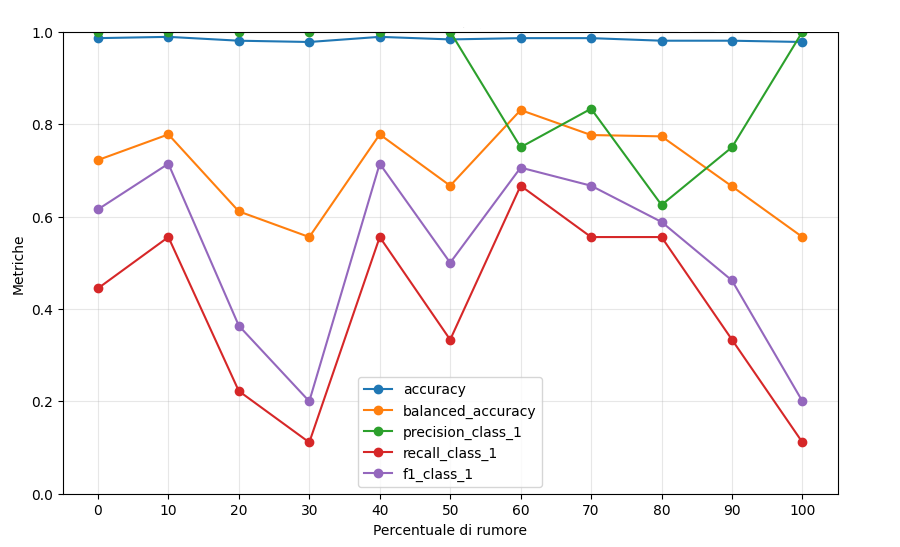
\includegraphics[width=1\textwidth]{Immagini/Teen/RobustezzaEnsamble2teen.png}%
    }
    \label{fig:alberiMiglioriDC}
\end{figure}



\begin{table}[h]
\centering
\label{tab:rumore_risultati}
\begin{tabular}{cccccc}
\hline
\textbf{\% Rumore} & \textbf{Accuracy} & \textbf{Balanced Acc.} & \textbf{Precision} & \textbf{Recall} & \textbf{F1} \\ 
\hline
0   & 0.9861 & 0.7222 & 1.0000 & 0.4444 & 0.6154 \\
10  & 0.9889 & 0.7778 & 1.0000 & 0.5556 & 0.7143 \\
20  & 0.9806 & 0.6111 & 1.0000 & 0.2222 & 0.3636 \\
30  & 0.9778 & 0.5556 & 1.0000 & 0.1111 & 0.2000 \\
40  & 0.9889 & 0.7778 & 1.0000 & 0.5556 & 0.7143 \\
50  & 0.9833 & 0.6667 & 1.0000 & 0.3333 & 0.5000 \\
60  & 0.9861 & 0.8305 & 0.7500 & 0.6667 & 0.7059 \\
70  & 0.9861 & 0.7764 & 0.8333 & 0.5556 & 0.6667 \\
80  & 0.9806 & 0.7735 & 0.6250 & 0.5556 & 0.5882 \\
90  & 0.9806 & 0.6652 & 0.7500 & 0.3333 & 0.4615 \\
100 & 0.9778 & 0.5556 & 1.0000 & 0.1111 & 0.2000 \\
\hline
\end{tabular}
\caption{Risultati ottenuti dal Decision Tree sporcando le feature migliori}
\end{table}


\subsubsection{Neural Network}

\begin{figure}[H]
    \centering
    \makebox[\textwidth][c]{%
        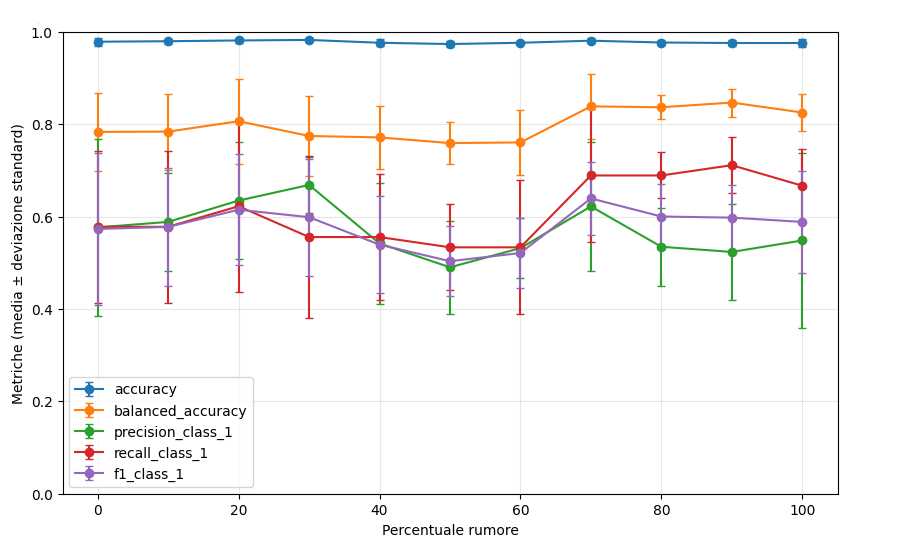
\includegraphics[width=1\textwidth]{Immagini/Teen/RobustezzaNNEnsembleTeen.png}%
    }
    \label{fig:alberiPeggioriNNTeen}
\end{figure}

\begin{table}[h]
\centering
\label{tab:rumore_risultati_3}
\begin{tabular}{cccccc}
\hline
\textbf{\%} Rumore& \textbf{Accuracy} & \textbf{Balanced Acc.} & \textbf{Precision} & \textbf{Recall} & \textbf{F1} \\
\hline
0   & 0.9783 & 0.7832 & 0.5765 & 0.5778 & 0.5730 \\
10  & 0.9794 & 0.7838 & 0.5884 & 0.5778 & 0.5776 \\
20  & 0.9811 & 0.8063 & 0.6345 & 0.6222 & 0.6147 \\
30  & 0.9822 & 0.7744 & 0.6683 & 0.5556 & 0.5986 \\
40  & 0.9761 & 0.7712 & 0.5417 & 0.5556 & 0.5391 \\
50  & 0.9733 & 0.7590 & 0.4900 & 0.5333 & 0.5033 \\
60  & 0.9761 & 0.7604 & 0.5316 & 0.5333 & 0.5210 \\
70  & 0.9806 & 0.8385 & 0.6219 & 0.6889 & 0.6391 \\
80  & 0.9767 & 0.8365 & 0.5345 & 0.6889 & 0.6000 \\
90  & 0.9756 & 0.8467 & 0.5233 & 0.7111 & 0.5976 \\
100 & 0.9756 & 0.8251 & 0.5482 & 0.6667 & 0.5883 \\
\hline
\end{tabular}
\caption{Risultati ottenuti dalla NN sporcando le feature peggiori}
\end{table}

\begin{figure}[H]
    \centering
    \makebox[\textwidth][c]{%
        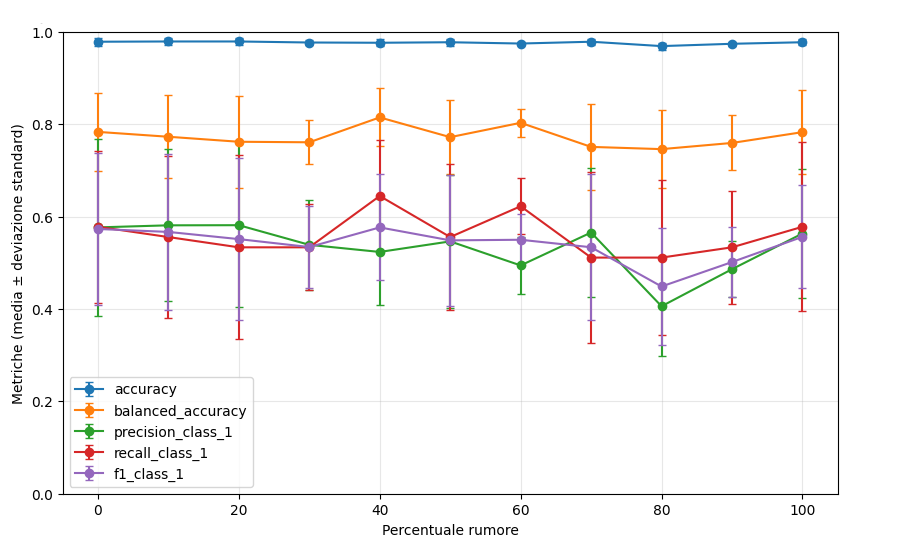
\includegraphics[width=1\textwidth]{Immagini/Teen/RobustezzaNN2EnsembleTeen.png}%
    }
    \label{fig:alberiMiglioriNNTeen}
\end{figure}

\begin{table}[h]
\centering
\label{tab:rumore_risultati_2}
\begin{tabular}{cccccc}
\hline
\textbf{\% Rumore} & \textbf{Accuracy} & \textbf{Balanced Acc.} & \textbf{Precision} & \textbf{Recall} & \textbf{F1} \\
\hline
0   & 0.9783 & 0.7832 & 0.5765 & 0.5778 & 0.5730 \\
10  & 0.9789 & 0.7727 & 0.5810 & 0.5556 & 0.5667 \\
20  & 0.9789 & 0.7618 & 0.5812 & 0.5333 & 0.5511 \\
30  & 0.9767 & 0.7607 & 0.5387 & 0.5333 & 0.5339 \\
40  & 0.9761 & 0.8145 & 0.5233 & 0.6444 & 0.5764 \\
50  & 0.9772 & 0.7718 & 0.5462 & 0.5556 & 0.5484 \\
60  & 0.9744 & 0.8028 & 0.4941 & 0.6222 & 0.5497 \\
70  & 0.9783 & 0.7507 & 0.5654 & 0.5111 & 0.5335 \\
80  & 0.9689 & 0.7459 & 0.4058 & 0.5111 & 0.4486 \\
90  & 0.9739 & 0.7593 & 0.4860 & 0.5333 & 0.5014 \\
100 & 0.9772 & 0.7826 & 0.5632 & 0.5778 & 0.5561 \\
\hline
\end{tabular}
\caption{Risultati ottenuti dalla NN sporcando le feature migliori}
\end{table}

\subsubsection{SVM}



\begin{figure}[H]
    \centering
    \makebox[\textwidth][c]{%
        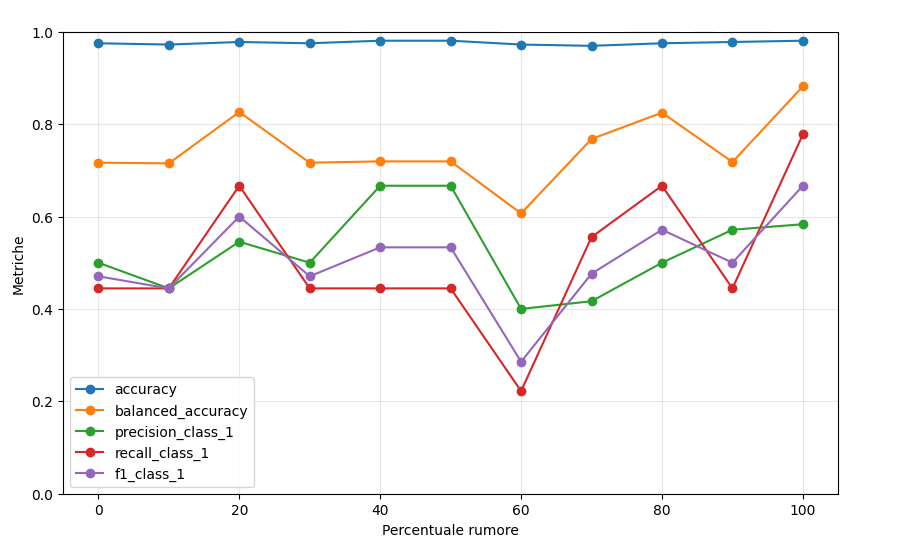
\includegraphics[width=1\textwidth]{Immagini/Teen/RobustezzaSVMEnsemble1.png}%
    }
    \label{fig:alberiPeggioriSVMTeen}
\end{figure}

\begin{table}[h]
\centering
\label{tab:rumore_risultati_5}
\begin{tabular}{cccccc}
\hline
\textbf{\% Rumore} & \textbf{Accuracy} & \textbf{Balanced Acc.} & \textbf{Precision} & \textbf{Recall} & \textbf{F1} \\
\hline
0   & 0.9750 & 0.7165 & 0.5000 & 0.4444 & 0.4706 \\
10  & 0.9722 & 0.7151 & 0.4444 & 0.4444 & 0.4444 \\
20  & 0.9778 & 0.8262 & 0.5455 & 0.6667 & 0.6000 \\
30  & 0.9750 & 0.7165 & 0.5000 & 0.4444 & 0.4706 \\
40  & 0.9806 & 0.7194 & 0.6667 & 0.4444 & 0.5333 \\
50  & 0.9806 & 0.7194 & 0.6667 & 0.4444 & 0.5333 \\
60  & 0.9722 & 0.6068 & 0.4000 & 0.2222 & 0.2857 \\
70  & 0.9694 & 0.7678 & 0.4167 & 0.5556 & 0.4762 \\
80  & 0.9750 & 0.8248 & 0.5000 & 0.6667 & 0.5714 \\
90  & 0.9778 & 0.7179 & 0.5714 & 0.4444 & 0.5000 \\
100 & 0.9806 & 0.8818 & 0.5833 & 0.7778 & 0.6667 \\
\hline
\end{tabular}
\caption{Risultati ottenuti dalla SVM sporcando le feature peggiori}
\end{table}


\begin{figure}[H]
    \centering
    \makebox[\textwidth][c]{%
        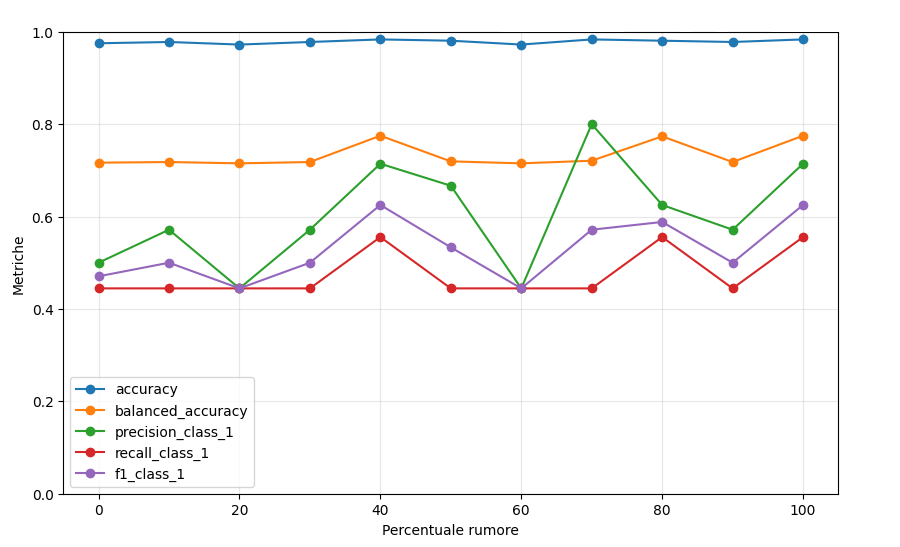
\includegraphics[width=1\textwidth]{Immagini/Teen/RobustezzaSVMEnsemble2.png}%
    }
    \label{fig:alberiMiglioriSVMTeen}
\end{figure}

\begin{table}[H]
\centering
\label{tab:rumore_risultati_4}
\begin{tabular}{cccccc}
\hline
\textbf{\% Rumore} & \textbf{Accuracy} & \textbf{Balanced Acc.} & \textbf{Precision} & \textbf{Recall} & \textbf{F1} \\
\hline
0   & 0.9750 & 0.7165 & 0.5000 & 0.4444 & 0.4706 \\
10  & 0.9778 & 0.7179 & 0.5714 & 0.4444 & 0.5000 \\
20  & 0.9722 & 0.7151 & 0.4444 & 0.4444 & 0.4444 \\
30  & 0.9778 & 0.7179 & 0.5714 & 0.4444 & 0.5000 \\
40  & 0.9833 & 0.7749 & 0.7143 & 0.5556 & 0.6250 \\
50  & 0.9806 & 0.7194 & 0.6667 & 0.4444 & 0.5333 \\
60  & 0.9722 & 0.7151 & 0.4444 & 0.4444 & 0.4444 \\
70  & 0.9833 & 0.7208 & 0.8000 & 0.4444 & 0.5714 \\
80  & 0.9806 & 0.7735 & 0.6250 & 0.5556 & 0.5882 \\
90  & 0.9778 & 0.7179 & 0.5714 & 0.4444 & 0.5000 \\
100 & 0.9833 & 0.7749 & 0.7143 & 0.5556 & 0.6250 \\
\hline
\end{tabular}
\caption{Risultati ottenuti dalla SVM sporcando le feature migliori}
\end{table}


\newpage
\section{Adult Income Dataset}

Il dataset vuole mostrare come il reddito annuo di un individuo dipende da diversi fattori. In modo intuitivo, è influenzato dal livello di istruzione, dall’età, dal genere, dall’occupazione e così via.

\subsection{Descrizione dataset}
Il dataset è composto da \textbf{15 colonne} e \textbf{48842 righe}.

\begin{table}[htbp]
\centering
\label{tab:featuresAdult}
\begin{tabular}{ll}
\hline
\textbf{Nome Variabile} & \textbf{Descrizione} \\
\hline
age & Età dell’individuo \\
workclass & Tipo di impiego \\
fnlwgt & Peso del campione censuario \\
education & Livello di istruzione, codificato come stringa \\
educational-num & Livello di istruzione, codificato come numero \\
marital-status & Stato civile \\
occupation & Occupazione \\
relationship & Relazione familiare \\
race & Razza \\
gender & Genere \\
capital-gain & Guadagni di capitale \\
capital-loss & Perdite di capitale \\
hours-per-week & Ore lavorate a settimana \\
native-country & Paese di origine \\
income & Variabile target (reddito annuo) \\
\hline
\end{tabular}
\end{table}

La distribuzione del target è: \textbf{76\% $\geq$ 50K, 24\% $<$ 50K}.

\begin{figure}[H]
    \centering
    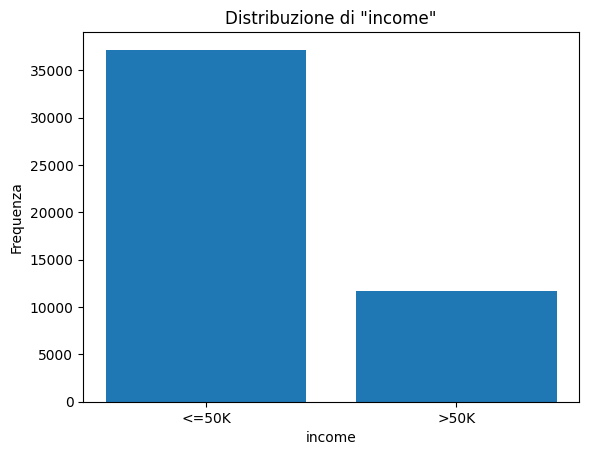
\includegraphics[width=0.75\linewidth]{Immagini/Adult/DistribuzioneTargetAdult.png}
    \label{fig:DistribuzioneTargetAdult}
\end{figure}

Attraverso il calcolo della Mutual Information per le varie feature, otteniamo una classifica, dalla più importante alla meno importante.

\begin{figure}[H]
    \centering
    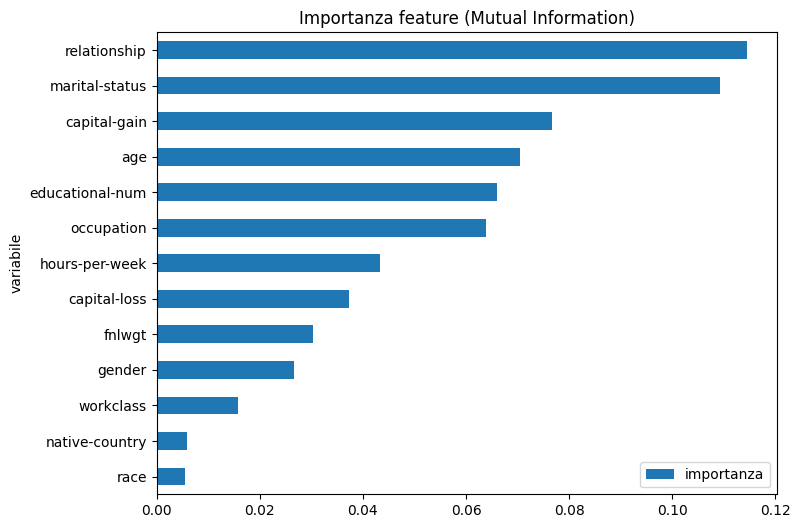
\includegraphics[width=1\linewidth]{Immagini/Adult/MIAdult.png}
    \label{fig:importanzaFeatureliver2}
\end{figure}



\subsection{Risultati}

\subsubsection{Decision Tree}

Dalla Mutual Information, otteniamo le 2 metà di feature:
\begin{itemize}
    \item \textbf{Peggiori}: ['hours-per-week', 'capital-loss', 'fnlwgt', 'gender', 'workclass', 'native-country', 'race'];
    \item \textbf{Migliori}: ['relationship', 'marital-status', 'capital-gain', 'age', 'educational-num', 'occupation', 'hours-per-week'].

\end{itemize}

\begin{figure}[H]
    \centering
    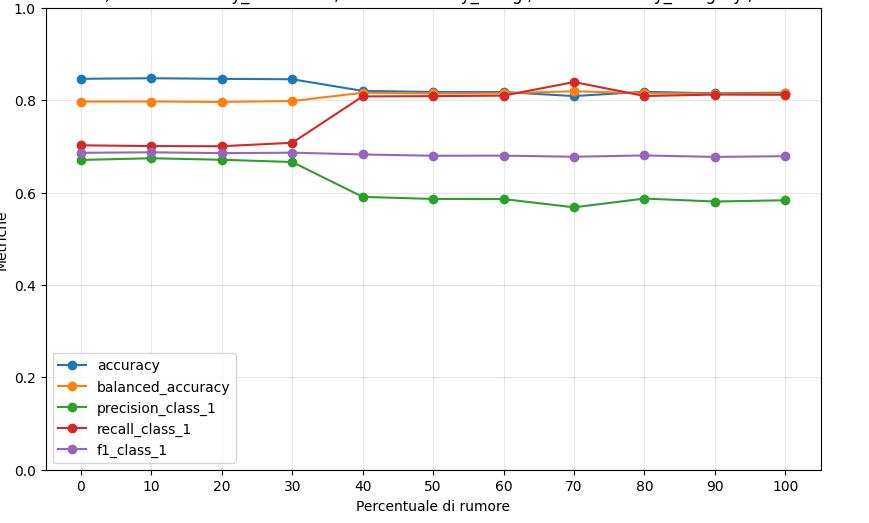
\includegraphics[width=1\linewidth]{Immagini/Adult/RobustezzaEnsemblePeggiori.jpeg}
    \label{fig:adult-robustezza-decision-tree-peggiori}
\end{figure}

\begin{table}[ht]
\centering
\begin{tabular}{cccccc}
\hline
\textbf{\% Rumore} & \textbf{Accuracy} & \textbf{Balanced Acc.} & \textbf{Precision} & \textbf{Recall} & \textbf{F1} \\
\hline
0   & 0.846 & 0.797 & 0.670 & 0.702 & 0.686 \\
10  & 0.847 & 0.797 & 0.674 & 0.701 & 0.687 \\
20  & 0.846 & 0.796 & 0.671 & 0.700 & 0.685 \\
30  & 0.845 & 0.798 & 0.666 & 0.708 & 0.686 \\
40  & 0.820 & 0.816 & 0.591 & 0.808 & 0.682 \\
50  & 0.818 & 0.815 & 0.586 & 0.809 & 0.680 \\
60  & 0.818 & 0.815 & 0.586 & 0.810 & 0.680 \\
70  & 0.809 & 0.819 & 0.568 & 0.839 & 0.677 \\
80  & 0.818 & 0.815 & 0.587 & 0.809 & 0.680 \\
90  & 0.815 & 0.814 & 0.581 & 0.812 & 0.677 \\
100 & 0.816 & 0.815 & 0.583 & 0.811 & 0.679 \\
\hline
\end{tabular}
\caption{Risultati ottenuti dal Decision Tree sporcando le feature peggiori}
\label{tab:prestazioni_feature_peggiori}
\end{table}

\begin{figure}[H]
    \centering
    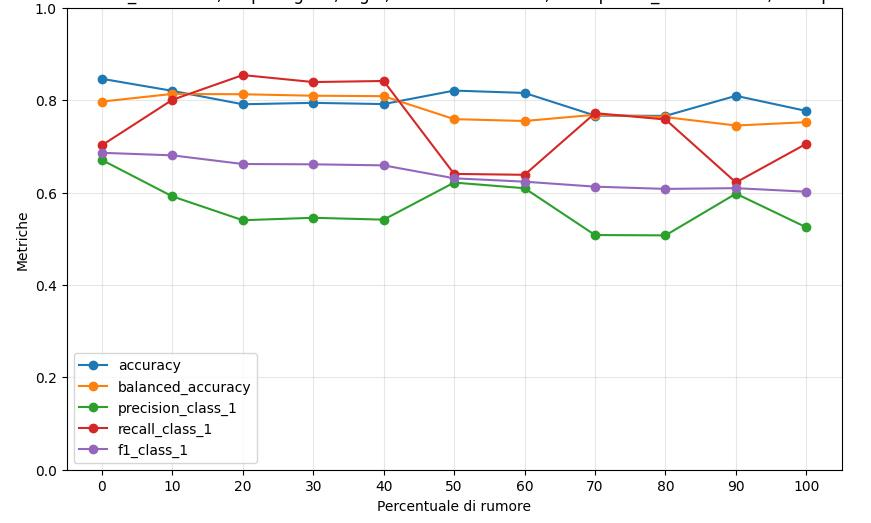
\includegraphics[width=1\linewidth]{Immagini/Adult/RobustezzaEnsembleMigliori.jpeg}
    \label{fig:adult-robustezza-decision-tree-migliori}
\end{figure}

\begin{table}[ht]
\centering
\begin{tabular}{cccccc}
\hline
\textbf{\% Rumore} & \textbf{Accuracy} & \textbf{Balanced Acc.} & \textbf{Precision} & \textbf{Recall} & \textbf{F1} \\
\hline
0   & 0.846 & 0.797 & 0.670 & 0.702 & 0.686 \\
10  & 0.820 & 0.813 & 0.592 & 0.801 & 0.680 \\
20  & 0.791 & 0.813 & 0.540 & 0.854 & 0.662 \\
30  & 0.794 & 0.810 & 0.545 & 0.839 & 0.661 \\
40  & 0.791 & 0.809 & 0.541 & 0.841 & 0.659 \\
50  & 0.821 & 0.759 & 0.622 & 0.640 & 0.631 \\
60  & 0.816 & 0.755 & 0.609 & 0.638 & 0.623 \\
70  & 0.767 & 0.768 & 0.508 & 0.772 & 0.613 \\
80  & 0.766 & 0.763 & 0.507 & 0.758 & 0.608 \\
90  & 0.809 & 0.745 & 0.598 & 0.622 & 0.609 \\
100 & 0.777 & 0.752 & 0.525 & 0.706 & 0.602 \\
\hline
\end{tabular}
\caption{Risultati ottenuti dal Decision Tree sporcando le feature migliori}
\label{tab:prestazioni_feature_migliori}
\end{table}

\subsubsection{Neural Network}


\begin{figure}[H]
    \centering
    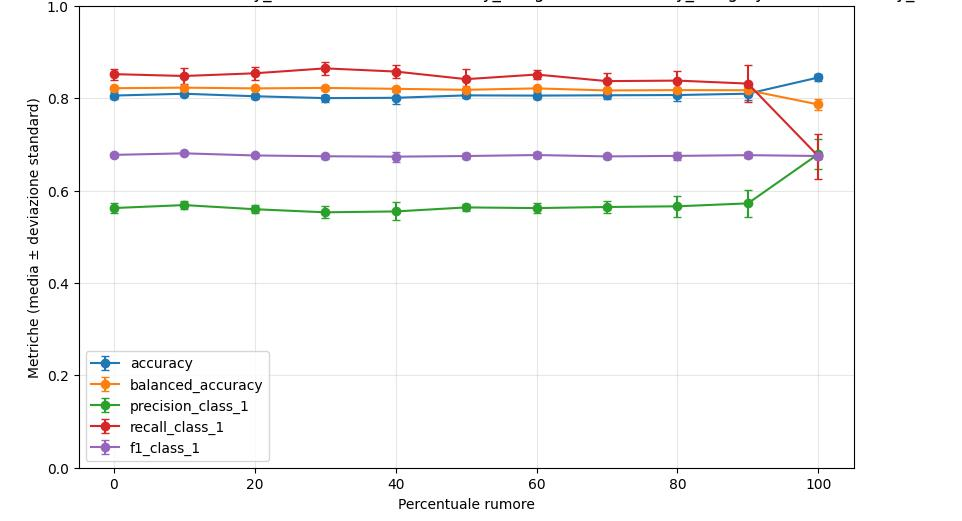
\includegraphics[width=1\linewidth]{Immagini/Adult/RobustezzaNNPeggiori.jpeg}
    \label{fig:adult-robustezza-nn-peggiori}
\end{figure}

\begin{table}[ht]
\centering
\begin{tabular}{cccccc}
\hline
\textbf{\% Rumore} & \textbf{Accuracy} & \textbf{Balanced Acc.} & \textbf{Precision} & \textbf{Recall} & \textbf{F1} \\
\hline
0   & 0.806 & 0.821 & 0.562 & 0.852 & 0.677 \\
10  & 0.809 & 0.823 & 0.568 & 0.848 & 0.680 \\
20  & 0.804 & 0.821 & 0.560 & 0.854 & 0.676 \\
30  & 0.800 & 0.822 & 0.553 & 0.864 & 0.674 \\
40  & 0.801 & 0.820 & 0.555 & 0.858 & 0.673 \\
50  & 0.806 & 0.818 & 0.563 & 0.841 & 0.675 \\
60  & 0.805 & 0.821 & 0.562 & 0.851 & 0.677 \\
70  & 0.806 & 0.817 & 0.564 & 0.837 & 0.674 \\
80  & 0.807 & 0.817 & 0.566 & 0.838 & 0.675 \\
90  & 0.810 & 0.817 & 0.572 & 0.831 & 0.677 \\
100 & 0.845 & 0.786 & 0.679 & 0.674 & 0.675 \\
\hline
\end{tabular}
\caption{Risultati ottenuti dalla Neural Network sporcando le feature peggiori.}
\label{tab:prestazioni_feature_peggiori}
\end{table}

\begin{figure}[H]
    \centering
    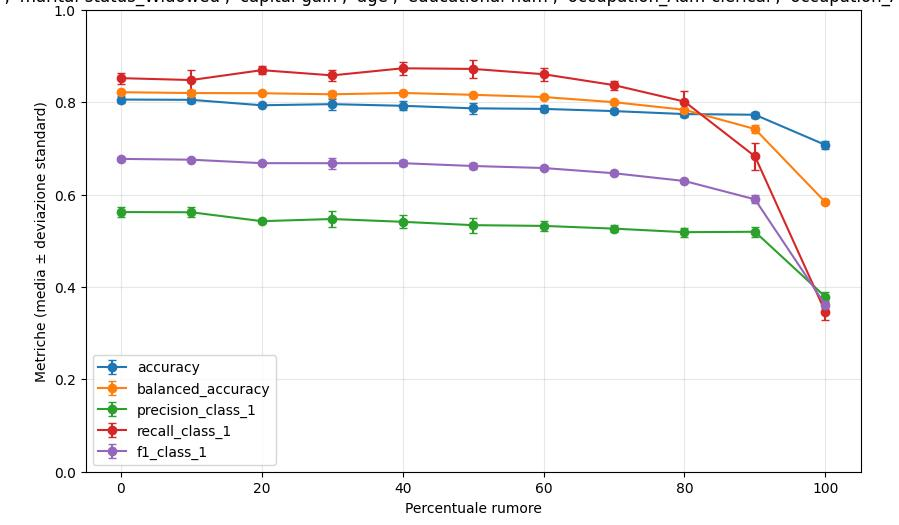
\includegraphics[width=1\linewidth]{Immagini/Adult/RobustezzaNNMigliori.jpeg}
    \label{fig:adult-robustezza-nn-migliori}
\end{figure}

\begin{table}[ht]
\centering
\begin{tabular}{cccccc}
\hline
\textbf{\% Rumore} & \textbf{Accuracy} & \textbf{Balanced Acc.} & \textbf{Precision} & \textbf{Recall} & \textbf{F1} \\
\hline
0   & 0.806 & 0.821 & 0.562 & 0.852 & 0.677 \\
10  & 0.805 & 0.820 & 0.562 & 0.848 & 0.675 \\
20  & 0.793 & 0.819 & 0.542 & 0.869 & 0.668 \\
30  & 0.796 & 0.817 & 0.547 & 0.858 & 0.668 \\
40  & 0.792 & 0.820 & 0.541 & 0.873 & 0.668 \\
50  & 0.787 & 0.816 & 0.534 & 0.872 & 0.662 \\
60  & 0.785 & 0.811 & 0.532 & 0.860 & 0.657 \\
70  & 0.781 & 0.800 & 0.526 & 0.837 & 0.646 \\
80  & 0.774 & 0.783 & 0.518 & 0.801 & 0.629 \\
90  & 0.773 & 0.742 & 0.519 & 0.683 & 0.590 \\
100 & 0.707 & 0.583 & 0.379 & 0.346 & 0.361 \\
\hline
\end{tabular}
\caption{Risultati ottenuti dalla Neural Network sporcando le feature migliori.}
\label{tab:prestazioni_feature_migliori}
\end{table}

\subsubsection{SVM}

\begin{figure}[H]
    \centering
    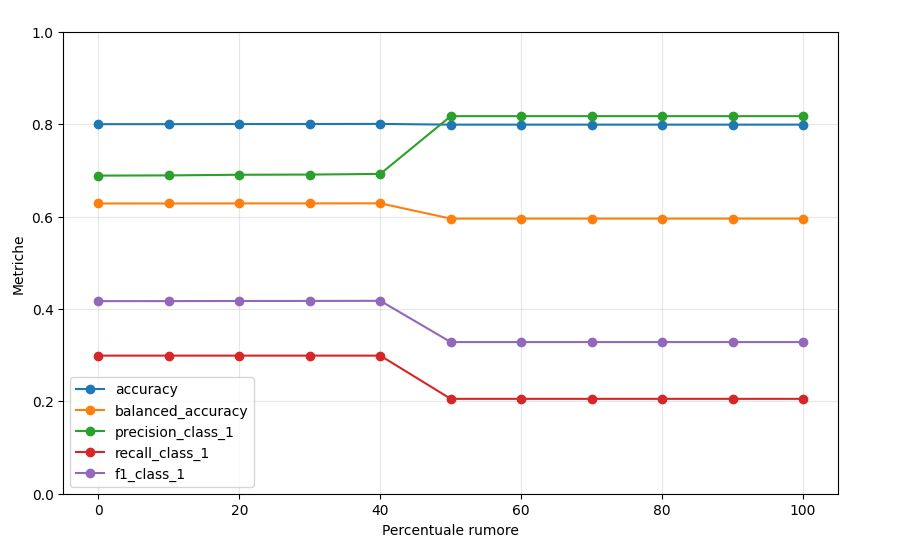
\includegraphics[width=1\linewidth]{Immagini/Adult/RobustezzaSVMPeggiori.png}
    \label{fig:adult-robustezza-svm-peggiori}
\end{figure}

\begin{table}[htbp]
\centering
\label{tab:rumore_risultati6}
\begin{tabular}{cccccc}
\hline
\textbf{\% Rumore} & \textbf{Accuracy} & \textbf{Balanced Acc.} & \textbf{Precision} & \textbf{Recall} & \textbf{F1} \\
\hline
0   & 0.7999 & 0.6282 & 0.6886 & 0.2989 & 0.4169 \\
10  & 0.8000 & 0.6282 & 0.6890 & 0.2989 & 0.4169 \\
20  & 0.8002 & 0.6284 & 0.6904 & 0.2989 & 0.4172 \\
30  & 0.8002 & 0.6284 & 0.6908 & 0.2989 & 0.4173 \\
40  & 0.8005 & 0.6286 & 0.6922 & 0.2989 & 0.4175 \\
50  & 0.7989 & 0.5955 & 0.8173 & 0.2054 & 0.3282 \\
60  & 0.7989 & 0.5955 & 0.8173 & 0.2054 & 0.3282 \\
70  & 0.7989 & 0.5955 & 0.8173 & 0.2054 & 0.3282 \\
80  & 0.7989 & 0.5955 & 0.8173 & 0.2054 & 0.3282 \\
90  & 0.7989 & 0.5955 & 0.8173 & 0.2054 & 0.3282 \\
100 & 0.7989 & 0.5955 & 0.8173 & 0.2054 & 0.3282 \\
\hline
\end{tabular}
\caption{Risultati ottenuti dalla SVM sporcando le feature peggiori}
\end{table}

\begin{figure}[H]
    \centering
    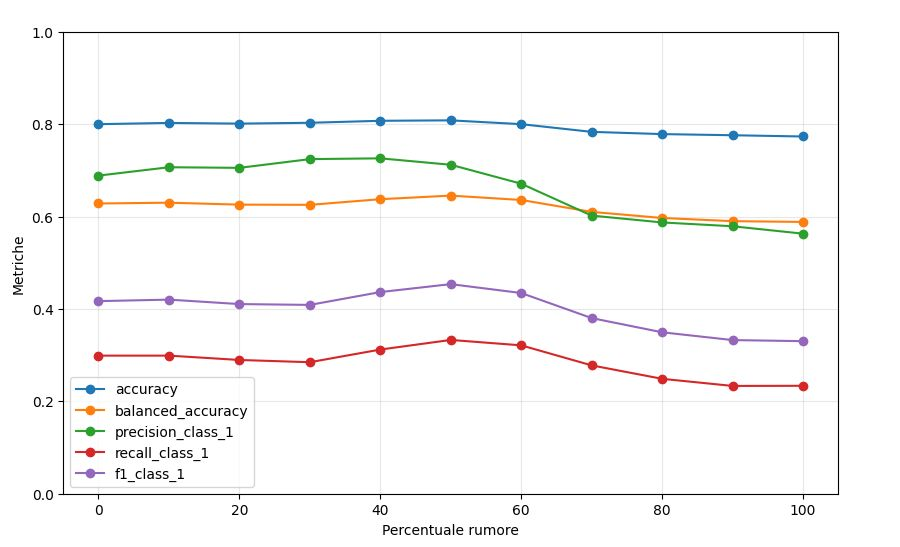
\includegraphics[width=1\linewidth]{Immagini/Adult/RobustezzaSVMMigliori.png}
    \label{fig:adult-robustezza-svm-migliori}
\end{figure}

\begin{table}[htbp]
\centering
\label{tab:rumore_risultati7}
\begin{tabular}{cccccc}
\hline
\textbf{\% Rumore} & \textbf{Accuracy} & \textbf{Balanced Acc.} & \textbf{Precision} & \textbf{Recall} & \textbf{F1} \\
\hline
0   & 0.7999 & 0.6282 & 0.6886 & 0.2989 & 0.4169 \\
10  & 0.8026 & 0.6299 & 0.7067 & 0.2989 & 0.4201 \\
20  & 0.8011 & 0.6257 & 0.7054 & 0.2895 & 0.4105 \\
30  & 0.8029 & 0.6253 & 0.7242 & 0.2847 & 0.4087 \\
40  & 0.8072 & 0.6375 & 0.7259 & 0.3120 & 0.4365 \\
50  & 0.8082 & 0.6453 & 0.7120 & 0.3329 & 0.4536 \\
60  & 0.7999 & 0.6358 & 0.6710 & 0.3212 & 0.4344 \\
70  & 0.7833 & 0.6100 & 0.6020 & 0.2778 & 0.3802 \\
80  & 0.7784 & 0.5969 & 0.5872 & 0.2487 & 0.3494 \\
90  & 0.7760 & 0.5900 & 0.5789 & 0.2333 & 0.3326 \\
100 & 0.7732 & 0.5883 & 0.5629 & 0.2336 & 0.3302 \\
\hline
\end{tabular}
\caption{Risultati ottenuti dalla SVM sporcando le feature migliori}
\end{table}

\newpage

\section{Analisi dei Risultati}

Analizzando i vari output dei modelli, notiamo che, in generale, sporcare le feature migliori porta a una maggiore instabilità dei risultati rispetto a sporcare le feature peggiori.\\
Inoltre, in media, sporcare le feature migliori porta a risultati peggiori rispetto allo sporcare feature migliori.

\begin{figure}[ht]
    \centering

    \begin{subfigure}{0.48\textwidth}
        \centering
        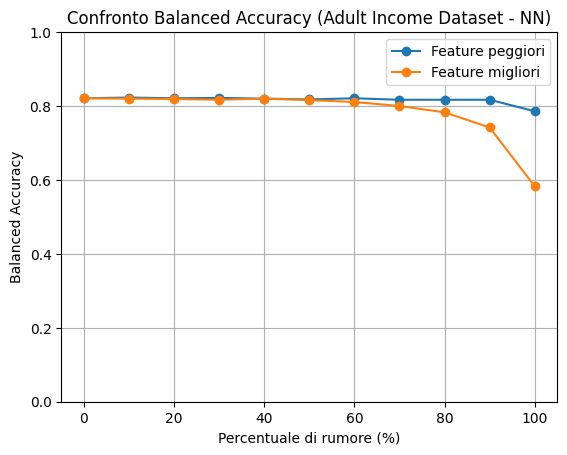
\includegraphics[width=\linewidth]{Immagini/Confronto/AID-NN.png}
        \label{fig:img1}
    \end{subfigure}
    \hfill
    \begin{subfigure}{0.48\textwidth}
        \centering
        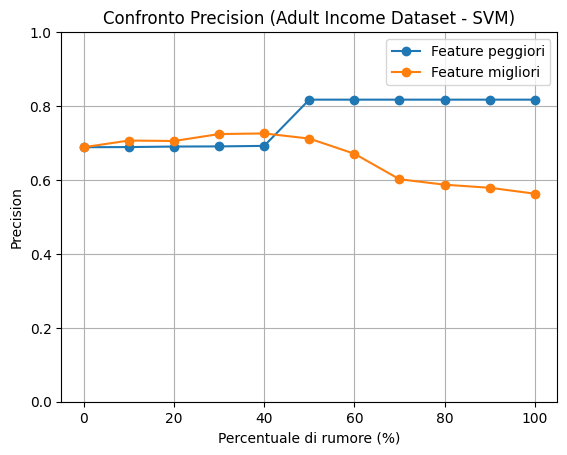
\includegraphics[width=\linewidth]{Immagini/Confronto/AID-SVM.png}
        \label{fig:img2}
    \end{subfigure}
    \label{fig:due_immagini}
\end{figure}
\begin{figure}[ht]
    \captionsetup{labelformat=empty}
    \centering

    \begin{subfigure}{0.48\textwidth}
        \centering
        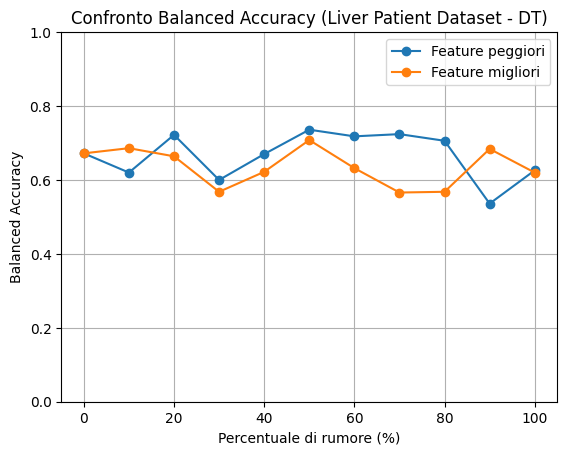
\includegraphics[width=\linewidth]{Immagini/Confronto/LPD-DT.png}
        \label{fig:img1}
    \end{subfigure}
    \hfill
    \begin{subfigure}{0.495\textwidth}
        \centering
        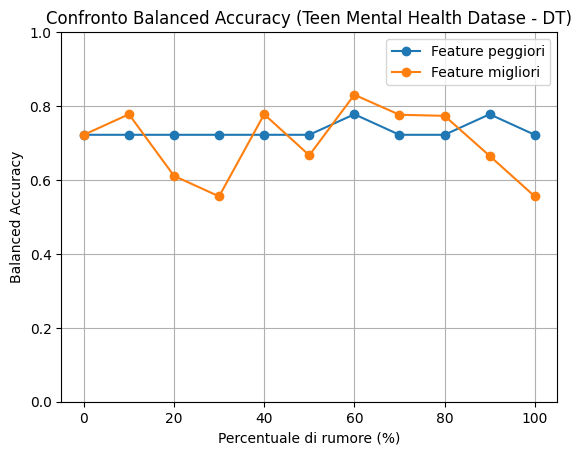
\includegraphics[width=\linewidth]{Immagini/Confronto/TMHD-DT.png}
        \label{fig:img2}
    \end{subfigure}

    \caption{Figura 1: Esempi di come sporcando le feature migliori, i risultati siano più instabili}
    \label{fig:due_immagini}
\end{figure}

\newpage
Dai nostri test, risulta che il Decision Tree, nel caso di Liver Patient Dataset e Teen Mental Health Dataset, è il modello più sensibile al rumore, mentre in Adult Income Dataset il modello più sensibile è la rete neurale, le cui prestazioni calano visibilmente a partire dall'80-90\% di rumore applicato. \\


\begin{figure}[H]
    \centering
    \captionsetup{labelformat=empty}

    \begin{subfigure}{0.48\textwidth}
        \centering
        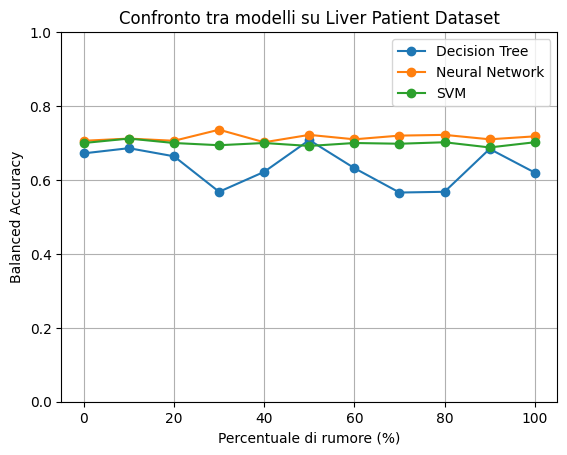
\includegraphics[width=\linewidth]{Immagini/Confronto/Liver.png}
        \label{fig:img1}
    \end{subfigure}
    \hfill
    \begin{subfigure}{0.48\textwidth}
        \centering
        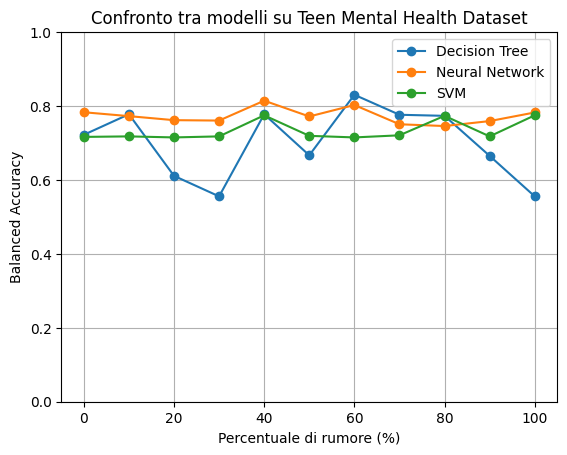
\includegraphics[width=\linewidth]{Immagini/Confronto/Teen.png}
        \label{fig:img2}
    \end{subfigure}
    \label{fig:due_immagini_2}
\end{figure}
\begin{figure}[H]
    \captionsetup{labelformat=empty}
    \centering
    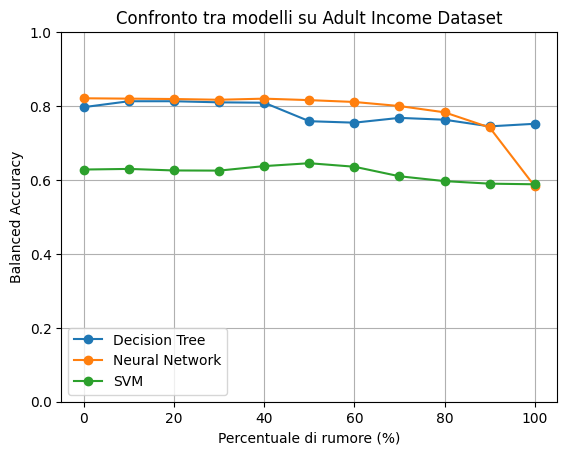
\includegraphics[width=0.5\linewidth]{Immagini/Confronto/Adult.png}
    \label{fig:confronto}

    \caption{Figura 2: Confronti fra modelli al variare del dataset, sporcando le feature migliori}
    \label{fig:due_immagini}
\end{figure}

Notiamo che l'unico dataset dove i risultati peggiorano sporcando le feature migliori, confrontando i risultati con lo 0\% di rumore con quelli con il 100\%, risulta essere Adult Income Dataset, che è il dataset con maggior numero di righe. \\
Infatti, nei dataset piccoli (come Liver Patient Dataset e Teen Mental Health Dataset) il rumore ha un effetto più instabile perché ogni campione ha un peso elevato e modificare anche pochi dati altera sensibilmente l’informazione complessiva. Nei dataset grandi, invece, lo stesso livello di rumore si distribuisce su molti più esempi e il suo impatto si attenua, rendendo il modello più stabile. Un ragionamento simile viene effettuato dal paper di ispirazione.

\newpage

Inoltre notiamo che, tra i dataset scelti, Teen Mental Health sembra essere quello più sensibile al rumore (presenta anche più valori di deviazione standard nella più elevati nelle reti neurali).

\begin{figure}[H]
    \centering
    \captionsetup{labelformat=empty}

    \begin{subfigure}{0.48\textwidth}
        \centering
        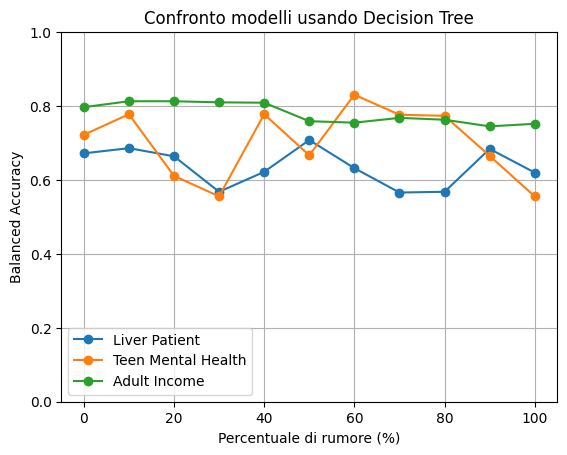
\includegraphics[width=\linewidth]{Immagini/Confronto/DT.png}
        \label{fig:img1}
    \end{subfigure}
    \hfill
    \begin{subfigure}{0.48\textwidth}
        \centering
        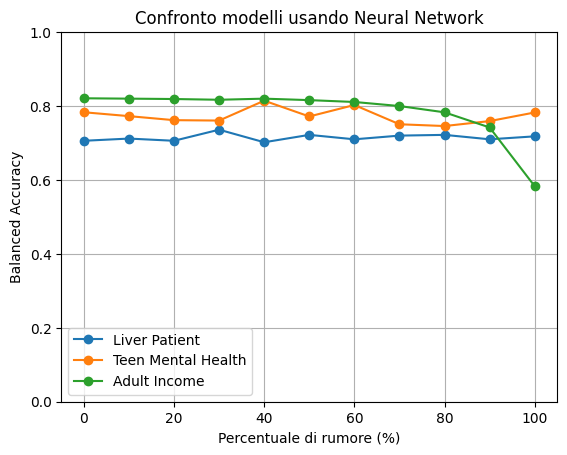
\includegraphics[width=\linewidth]{Immagini/Confronto/NN.png}
        \label{fig:img2}
    \end{subfigure}
    \label{fig:due_immagini_2}
\end{figure}
\begin{figure}[H]
    \captionsetup{labelformat=empty}
    \centering
    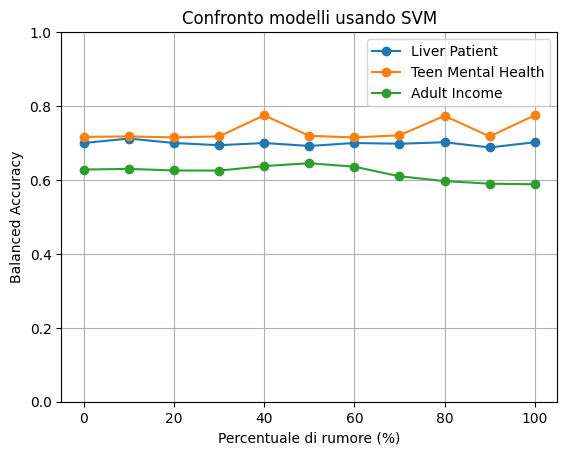
\includegraphics[width=0.5\linewidth]{Immagini/Confronto/SVM.png}
    \label{fig:confronto}

    \caption{Figura 3: Confronti fra Dataset al variare del modello, sporcando le feature migliori}
    \label{fig:due_immagini}
\end{figure}



Si osserva infine un aspetto rilevante: la noise injection è una metodologia ampiamente studiata in letteratura come tecnica di regolarizzazione. Nei risultati ottenuti, l’introduzione di rumore non porta sempre ad un peggioramento delle prestazioni; al contrario, in diversi casi si osserva un miglioramento delle  metriche discusse all’aumentare controllato dell’intensità del rumore. Tale comportamento è coerente con l’interpretazione della noise injection come meccanismo di regolarizzazione, in grado di indurre rappresentazioni più robuste, ridurre l’overfitting su strutture locali potenzialmente non affidabili e favorire una maggiore stabilità del processo di apprendimento.\\
Questo aiuta il modello a non adattarsi troppo ai dettagli del training set e quindi a funzionare meglio anche su dati nuovi, migliorando la capacità di generalizzazione.


\newpage
\section{Conclusioni}
In questo progetto abbiamo analizzato come il rumore influisca sull’addestramento di:
\begin{enumerate}
    \item Decision Tree,
    \item Neural Network,
    \item SVM,
\end{enumerate}


con 3 dataset differenti.
Abbiamo mostrato i vari risultati ottenuti e fatto qualche confronto degno di nota.
\par
Ulteriori esperimenti potrebbero concentrarsi sul confronto dei risultati ottenuti su dataset di dimensioni simili, così da valutare l'effetto del rumore indipendentemente dalla dimensione del dataset.\\
Inoltre, sarebbe interessante estendere l'analisi ad altri modelli di machine learning per verificarne il comportamento in presenza di rumore. \\
Si potrebbero testare anche diverse modalità di applicazione del rumore, al fine di individuare le strategie più efficaci.\\
Infine, si potrebbero testare altre misure per l’importanza delle feature per ottenere gruppi di feature da sporcare insieme.


\begin{thebibliography}{9}

\bibitem{Saseendran2019}
A.~T. Saseendran, L. Setia, V. Chhabria, D. Chakraborty, and A. Barman Roy.
\newblock \emph{Impact of Noise in Dataset on Machine Learning Algorithms}.
\newblock Machine Learning Research, 1:1--8, 2019.

\end{thebibliography}


\end{document}